\documentclass{article}
\usepackage{hyperref}
\hypersetup{
    bookmarks=true,                             % show bookmarks bar?
    unicode=false,                              % non-Latin characters in Acrobat's bookmarks
    pdftoolbar=true,                            % show Acrobat's toolbar?
    pdfmenubar=true,                            % show Acrobat's menu?
    pdffitwindow=true,                          % page fit to window when opened
    pdftitle={Smoothing polylines with circles},    % title
    pdfauthor={Jason Sewall},                   % author
    pdfsubject={}                      % subject of the document
    pdfcreator={},                       % creator of the document
    pdfproducer={},                     % producer of the document
    pdfkeywords={},                     % list of keywords
    pdfnewwindow=true,                          % links in new window
    colorlinks=true,                            % false: boxed links; true: colored links
    linkcolor=red,                              % color of internal links
    citecolor=blue,                             % color of links to bibliography
    filecolor=magenta,                          % color of file links
    urlcolor=cyan                               % color of external links
}
\usepackage{amsmath}
\usepackage{amssymb}
\usepackage[letterpaper]{geometry}
\usepackage{graphicx}
\usepackage{subfigure}
\title{Smoothing polylines with circles}
\author{Jason Sewall}
\date{October 4, 2009}
\begin{document}
\maketitle
%
\section{Smoothing two-dimensional polylines}
%
\subsection{The problem}
%
We have an ordered sequence $P$ of $n$ 2D points:
%
\begin{equation}
  \label{eq:points}
  P := \left(p_{0}, p_{1},\ldots,p_{n-2},p_{n-1}\right)
\end{equation}
%
These points define a (planar) polyline with $n-1$ segments such as that in Fig.~\ref{fig:polyline}.  Let us assume that there are no two points adjacent in the sequence that are equal, and that there are no three adjacent points that are colinear; clearly we can eliminate these adjacent repeated points or the central points in a colinear sequence without modifying the line's shape.
%
\begin{figure}[h]
  \centering
  \subfigure[\label{fig:polyline} A polyline $P$]{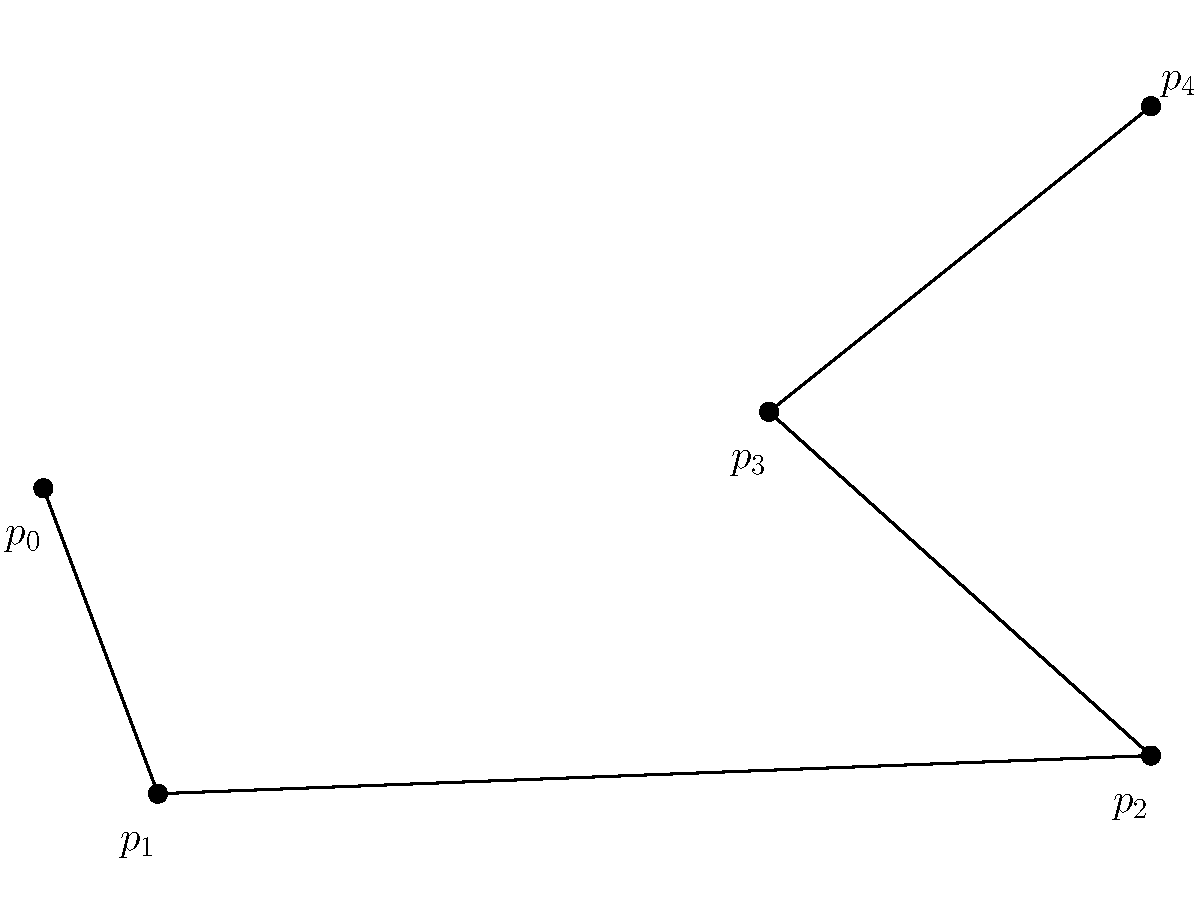
\includegraphics[width=7cm]{1}}\hfill
  \subfigure[\label{fig:smooth-polyline}$P_S$: A `smoothed' version of the polyline $P$]{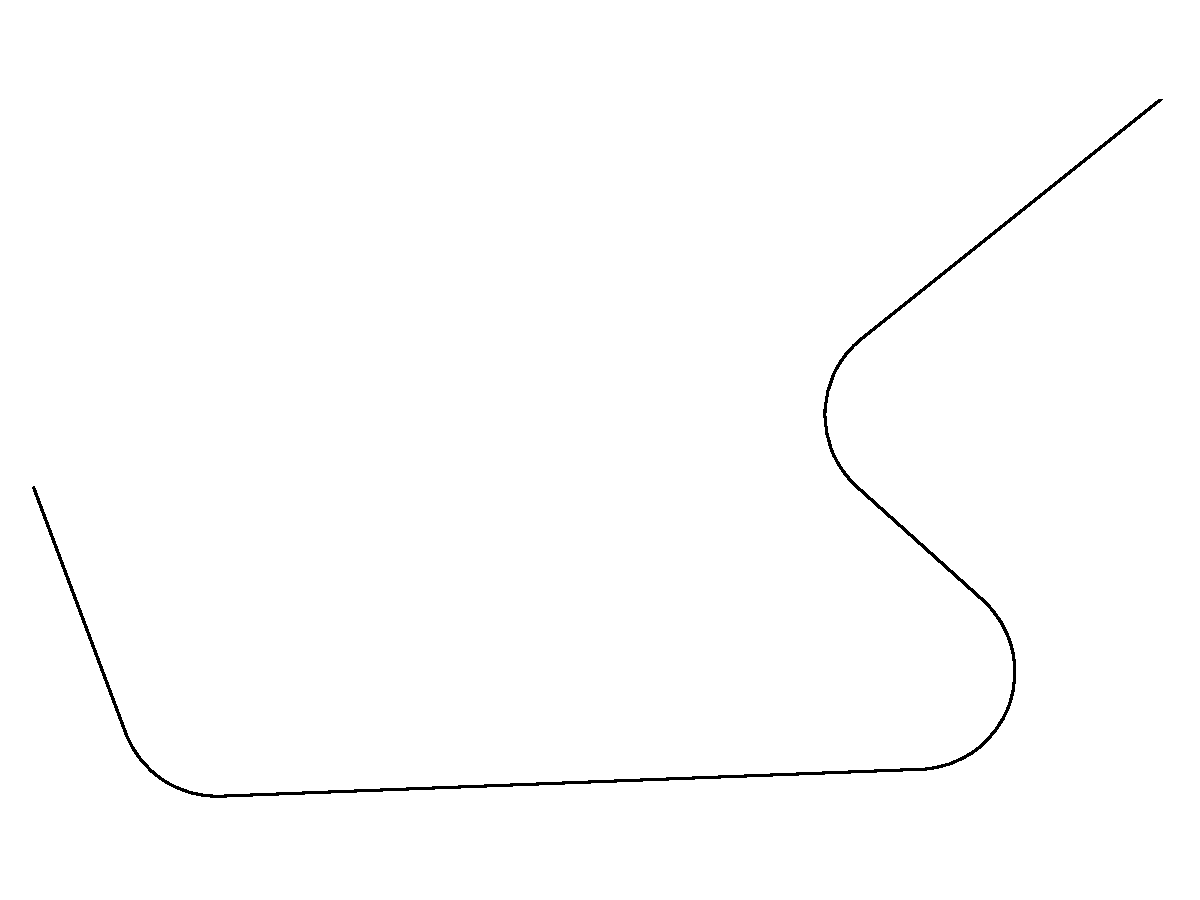
\includegraphics[width=7cm]{2}}\\
  \subfigure[\label{fig:debug-smooth-polyline}The polyline $P$ and the circles defining $P_S$]{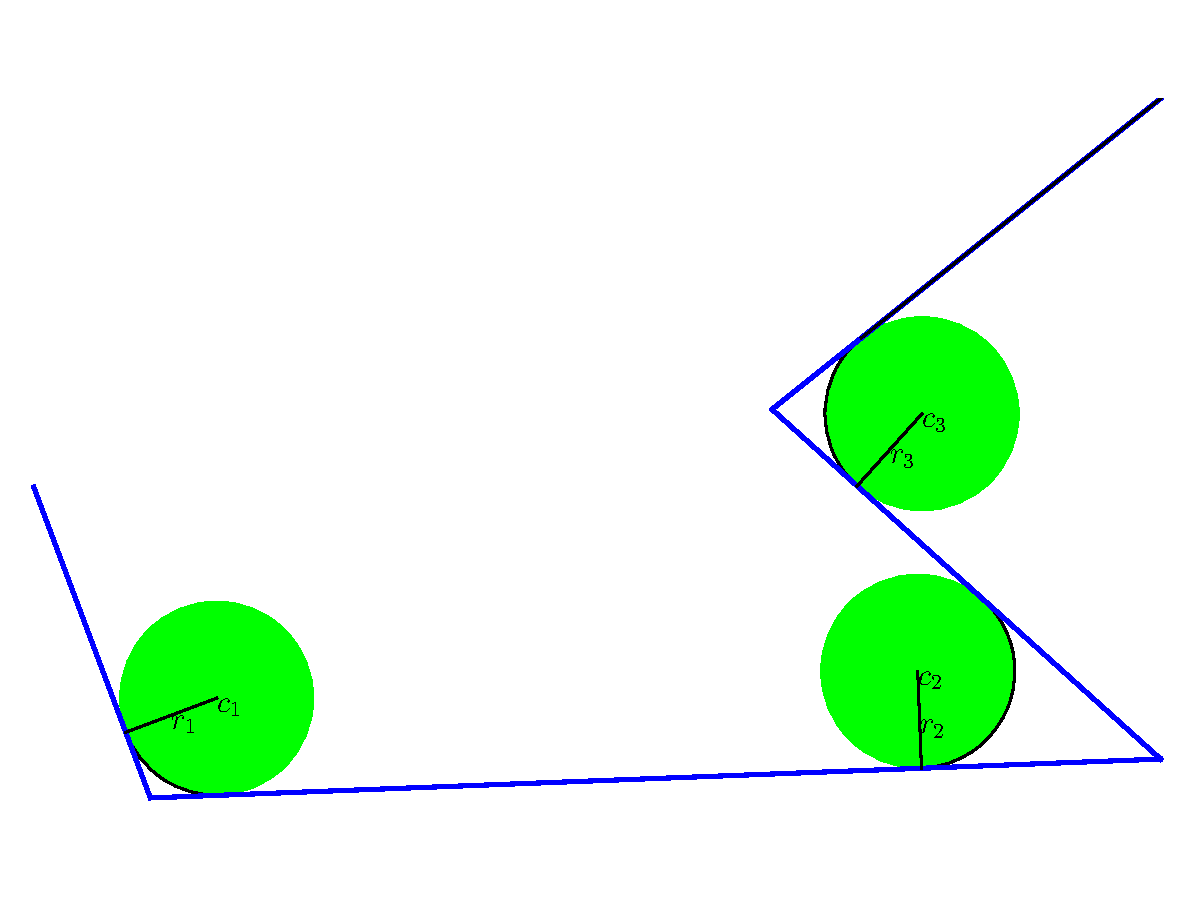
\includegraphics[width=7cm]{3}}
  \caption{Polylines}
\end{figure}
%
We wish to `smooth' this polyline to something like what is shown in Fig.~\ref{fig:smooth-polyline}, which we shall refer to as $P_S$.  We construct $P_S$ by replacing the region around each interior point $p_{i}, i \in \mathbb{Z}\left[1, n-2\right]$ of $P$ with a circular arc $\mathbf{a}_{i}$ and retaining the exterior points $p_0$ and $p_{n-1}$.  We abuse notation slightly and define
%
\begin{equation}
  \label{eq:p-smooth}
  P_S := \left(p_0, a_1, a_2, a_{n_2}, \ldots, p_{n-1}\right)
\end{equation}
%
Where each $\mathbf{a}_{i}$ is defined by:
%
\begin{equation}
  \label{eq:circ-def}
\mathbf{a}_i=\left(
  c_{i},
  r_{i},
  \phi^{0}_{i},
  \phi^{1}_{i}
\right)
\end{equation}
%
And here $c_{i}$ is the center, $r_{i}$ is the radius, and $\phi^{0}_{i}, \phi^{1}_{i}$ are the angular extents of the arc ordered such that the shortest arc from $\phi^0_i$ to $\phi^1_i$ begins at the tangent point on $\overline{p_{i-1}p_i}$ and ends on the tangent point to $\overline{p_ip_{i+1}}$.  See Fig. \ref{fig:debug-smooth-polyline}; each $\mathbf{a}_{i}$ is shown.
%
\subsection{Formulation of the arcs $a_{i}$}
\label{sec:formulation-arcs}
%
\subsubsection{Definitions}
%
For each interior point $p_{i}$, the associated arc $\mathbf{a}_{i}$ is determined closely associated with the triple of points:
%
\begin{equation}
  \label{eq:arc-triple}
  T_{i} = \left(p_{i-1}, p_{i}, p_{i+1}\right)
\end{equation}
%
\paragraph{Vectors}
%
In particular, we are interested in the derived vectors
%
\begin{align}
  \label{eq:vector-f}
  \mathbf{v}_{i} &= p_{i+1} - p_{i}
\end{align}
%
their lengths:
%
\begin{align}
  \label{eq:vector-length-f}
  L_{i} &= \left|\mathbf{v}_{i}\right|
\end{align}
%
and the associated unit vectors:
%
\begin{align}
  \label{eq:unit-vectors-f}
  \mathbf{n}_{i} &= \frac{\mathbf{v}_{i}}{L_{i}} =\frac{\mathbf{v}_{i}}{\left|\mathbf{v}_{i}\right|}
\end{align}
%
Henceforth, when performing computations with a $T_i$, we shall frequently refer to $-\mathbf{n}_{i-1} = \frac{p_{i-1}-p_i}{\left|p_{i-1}-p_i\right|}$.
%
\paragraph{Tangent points}
%
The projections of $c_{i}-p_{i}$ onto $-\mathbf{n}_{i-1}$ and onto $\mathbf{n}_{i}$ have equal length $\alpha_i$; then the tangent points of the circle on $-\mathbf{v}_{i-1}$ and $\mathbf{v}_{i}$ are:
%
\begin{align}
  \label{eq:alpha-vector-b}
  \left(c_{i}-p_{i}\right)\;\mathrm{proj}\; -\mathbf{n}_{i-1} &= -\alpha_i\mathbf{n}_{i-1}\\
  \label{eq:alpha-vector-f}
  \left(c_{i}-p_{i}\right)\;\mathrm{proj}\; \mathbf{n}_{i} &= \alpha_i\mathbf{n}_{i}
\end{align}
%
\paragraph{Radius vectors}
%
We are also interested in the (negative) radius vectors from these points to the center $c_{i}$:
%
\begin{align}
  \label{eq:radius-vector-b}
  \mathbf{r}^{-}_{i} &= c_{i} - \left(-\alpha\mathbf{n}_{i-1} + p_{i}\right)=c_{i} + \left(\alpha\mathbf{n}_{i-1} - p_{i}\right)&=\pm r_i\left(\mathbf{n}_{i-1}^{y},  -\mathbf{n}_{i-1}^{x} \right)\\
  \label{eq:radius-vector-f}
  \mathbf{r}^{+}_{i} &= c_{i} - \left(\alpha\mathbf{n}_{i} + p_{i}\right)&=\pm r_i\left(\mathbf{n}_{i}^{y}, -\mathbf{n}_{i}^{x} \right)
\end{align}
%
Obviously, $\left|\mathbf{r}^{-}_{i}\right| = \left|\mathbf{r}^{+}_{i}\right| = r_{i}$.

The sign of the rightmost term in Eqs.~\eqref{eq:radius-vector-b},~\eqref{eq:radius-vector-f} ($\pm$) is determined by the orientation of the triple $T_i$ (see Eq.~\eqref{eq:vector-f}); that is to say:
%
\begin{equation}
  \label{eq:orientation}
  o_i = \mathrm{sign}\; -\mathbf{n}_{i-1} \times \mathbf{n}_{i}
\end{equation}
%
\paragraph{The center}
%
The center $c_{i}$ can be determined by combining Eqs.~\eqref{eq:radius-vector-b},~\eqref{eq:radius-vector-f} and~\eqref{eq:alpha-vector-b}, ~\eqref{eq:alpha-vector-f}:
%
\begin{align}
  \label{eq:center-vector-b}
  c_{i} &= p_{i} - \alpha_i\mathbf{n}_{i-1} + \mathbf{r}^{-}_{i}\\
  \label{eq:center-vector-f}
  c_{i} &= p_{i} + \alpha_i\mathbf{n}_i + \mathbf{r}^{+}_{i}
\end{align}
%
We can also write $c_{i}$ in terms of the unit bisector $\mathbf{b}_{i}$:
%
\begin{equation}
  \label{eq:center-bisector}
  c_{i} = p_{i} + \sqrt{r_{i}^{2} + \alpha_{i}^{2}}\mathbf{b}_{i}
\end{equation}
%
Where $\mathbf{b}_i$ is of course given by:
%
\begin{equation}
  \label{eq:bisector}
  \mathbf{b}_i = \frac{\mathbf{n}_i-\mathbf{n}_{i-1}}{\left|\mathbf{n}_i-\mathbf{n}_{i-1}\right|}
\end{equation}
%
See Fig.~\ref{fig:interior-point} for a visual depiction of these quantities.
%
\begin{figure}[h]
  \centering
  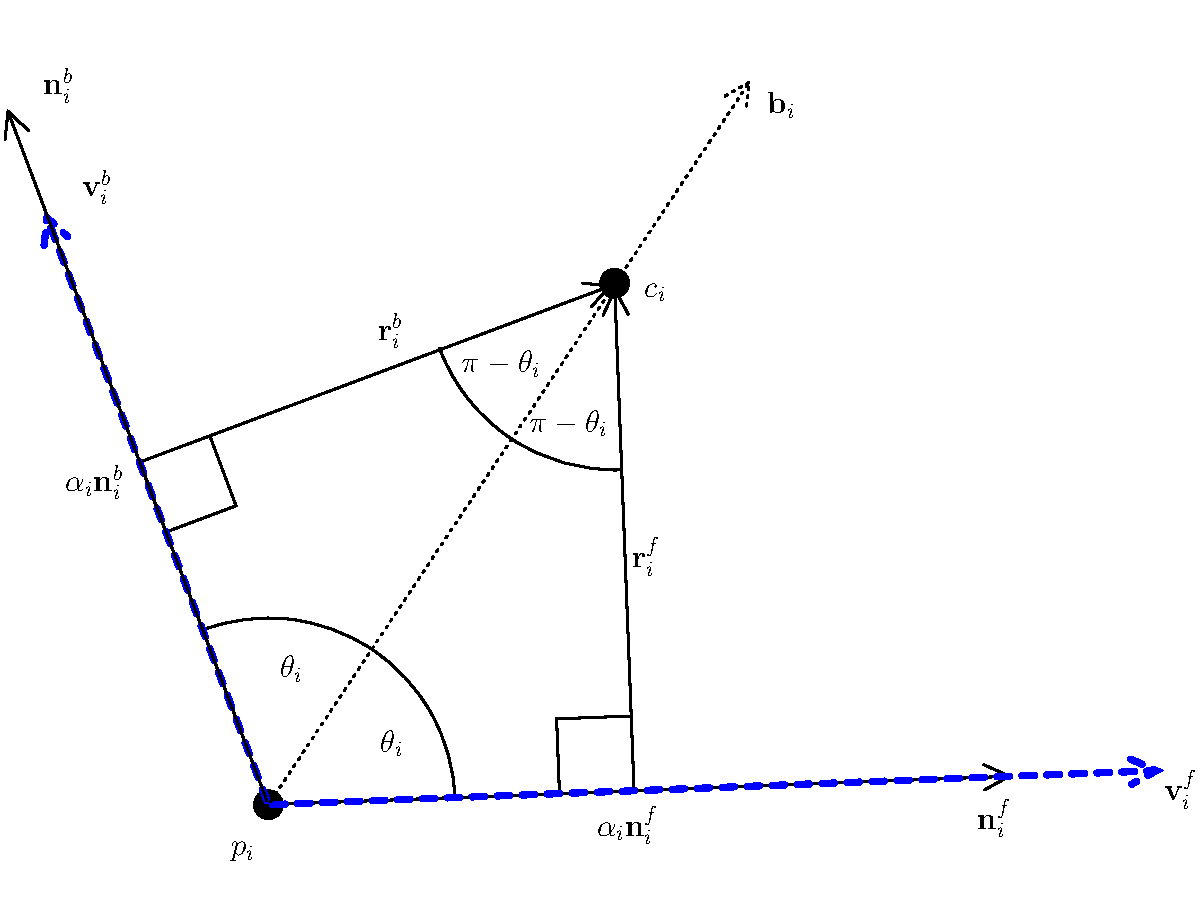
\includegraphics[width=\columnwidth]{4}
  \caption{The interior point $p_{i}$ with backward vector $-\mathbf{v}_{i-1}$ and forward vector $\mathbf{v}_{i}$. $\mathbf{b}_{i}$ is the unit bisector of these vectors}
  \label{fig:interior-point}
\end{figure}
%
x\subsubsection{Angles}
%
For a given $T_i$, the arc angles $\phi^0_i$ and $\phi^{1}_{i}$; are fixed regardless of the $c_i$ or $r_{i}$:
%
\begin{align}
  \label{eq:angle-range-b}
  \phi^{0}_{i} &= \arctan \frac{{\mathbf{r}^{-}_{i}}^{y}}{{\mathbf{r}^{-}_{i}}^{x}}\\
  \label{eq:angle-range-f}
  \phi^{1}_{i} &= \arctan \frac{{\mathbf{r}^{+}_{i}}^{y}}{{\mathbf{r}^{+}_{i}}^{x}}
\end{align}
%
The total arc length of $a_i$ (the angle $\left|\phi^0_i -\phi^1_i\right|$) is given by $2\left(\pi-\theta_i\right)$ (see Fig.~\ref{fig:interior-point})
%
We can also relate the input vectors for a given $T_{i}$ to $\theta$:
%
\begin{equation}
  \label{eq:dotnorm}
  -\mathbf{n}_{i-1} \cdot \mathbf{n}_i = \cos 2\theta_i
\end{equation}
%
Similarly, we know
%
\begin{align}
  \notag
  \left|\phi^0_i -\phi^1_i\right| &= 2\left(\pi-\theta_i\right)\\
  \notag
  &= 2\pi-\arccos -\mathbf{n}_{i-1} \cdot \mathbf{n}_i \\
  \notag
  &= 2\pi-\left(\arccos \mathbf{n}_{i-1} \cdot \mathbf{n}_i - \pi\right)\\
  \label{eq:arclen-dot}
  &= \pi-\arccos \mathbf{n}_{i-1} \cdot \mathbf{n}_i
\end{align}
%
Clearly, Eqs.~\eqref{eq:angle-range-b},~\eqref{eq:angle-range-f} and~\eqref{eq:dotnorm} are independent of other arc parameters $c_{i}$, $r_{i}$, and $\alpha_i$.
%
\subsubsection{Equation for $r_i$ and $\alpha_{i}$}
%
For a given triple $T_{i}$, we would like a formula relating $r_{i}$, and $\alpha_{i}$.  From visual inspection of Fig.~\ref{fig:interior-point}, we can see that:
%
\begin{align}
  \notag
  \frac{r_i}{\alpha_{i}} &= \tan \theta_i\\
  \label{eq:tantheta}
  r_i &= \alpha_{i}\tan \theta_i
\end{align}
%
We know from trigonometry that
%
\begin{align}
  \notag
  \tan \frac{s}{2} &= \sqrt{\frac{1-\cos s}{1+\cos s}}\\
  \label{eq:tanident}
  \tan \theta &= \sqrt{\frac{1-\cos 2\theta}{1+\cos 2\theta}}
\end{align}
%
We can combine Eq.~\eqref{eq:tantheta} with Eq.~\eqref{eq:tanident} to obtain
%
\begin{align}
  \label{eq:radiustan}
  r_{i} &= \alpha_i\sqrt{\frac{1-\cos 2\theta}{1+\cos 2\theta}}
\end{align}
%
Finally, we can substitute Eq.~\eqref{eq:dotnorm} into Eq.~\eqref{eq:radiustan}, and obtain
%
\begin{equation}
  \label{eq:radius-alpha}
  r_{i} = \alpha_i\sqrt{\frac{1-\mathbf{n}_i\cdot -\mathbf{n}_{i-1}}{1+\mathbf{n}_i\cdot -\mathbf{n}_{i-1}}} = \alpha_i\sqrt{\frac{1+\mathbf{n}_i\cdot \mathbf{n}_{i-1}}{1-\mathbf{n}_i\cdot \mathbf{n}_{i-1}}}
\end{equation}
%
\subsection{Length of a smoothed polyline}
\label{sec:length-smooth-polyl}
%
It is useful to consider the length of a smoothed polyline $P_S$.  This will be the sum of the circumference of each arc $a_i$ plus the length of the straight line segments connected consecutive arcs and the segments connecting $p_0$ to $a_1$ and $a_{n-2}$ to $p_{n-2}$.

The length $w_i$ of an arc $a_i = \left(c_i, r_i, \phi^0_i, \phi^1_i\right)$ is given by the standard formula:
%
\begin{equation}
  \label{eq:circumference}
  w_i  = 2\pi r_i \frac{\left|\phi^0_i - \phi^1_i\right|}{2\pi} = r_i \left|\phi^0_i - \phi^1_i\right|
\end{equation}
%
The length $s_i$ of a segment connecting two consecutive arcs $a_{i}$ and $a_{i+1}$ is simply the length of the original line from $p_i$ to $p_{i+1}$ ($L_i$) minus the $\alpha_i$ and $\alpha_{i+1}$ of $a_i$ and $a_{i+1}$:
%
\begin{equation}
  \label{eq:seglen}
  s_i = \left|p_{i+1} - p_{i}\right| - (\alpha_{i+1} + \alpha_{i}) = L_{i} - (\alpha_{i+1} + \alpha_{i})
\end{equation}
%
If we define $\alpha_0 = \alpha_{n-1} = 0$ for the endpoints $p_0$ and $p_{n-1}$, we can use Eq.~\eqref{eq:seglen} for the beginning/end segments as well.

For nondegenerate $P_S$ (i.e. with $n>2$), we have:
%
\begin{align}
  \notag
  L\left(P_S\right) &= \sum^{n-2}_{i = 1} r_i\left|\phi^0_i - \phi^1_i\right| + \sum^{n-2}_{i=0} s_i\\
  \notag
  &= \sum^{n-2}_{i = 1} r_i\left|\phi^0_i - \phi^1_i\right| + \sum^{n-2}_{i=0} L_i - (\alpha_{i+1} - \alpha_{i})\\
  \notag
  &= \sum^{n-2}_{i = 1} r_i\left|\phi^0_i - \phi^1_i\right| + L\left(P\right) - \sum^{n-2}_{i=0} \alpha_{i+1} - \sum^{n-2}_{i=0} \alpha_{i}\\
  \notag
  &= L\left(P\right) + \sum^{n-2}_{i = 1} r_i\left|\phi^0_i - \phi^1_i\right| - \sum^{n-1}_{i=1} \alpha_{i} - \sum^{n-2}_{i=0} \alpha_{i}\\
  \notag
  &= L\left(P\right) + \sum^{n-2}_{i = 1} r_i\left|\phi^0_i - \phi^1_i\right| - 2\sum^{n-2}_{i=1} \alpha_{i} - \alpha_0 - \alpha_{n-1}\\
  \label{eq:smoothpoly-len}
  &= L\left(P\right) + \sum^{n-2}_{i = 1} r_i\left|\phi^0_i - \phi^1_i\right| - 2\alpha_i
  % \notag
  % &= L\left(P\right) + \sum^{n-2}_{i = 1} \alpha_i\sqrt{\frac{1-\mathbf{n}_i\cdot -\mathbf{n}_{i-1}}{1+\mathbf{n}_i\cdot -\mathbf{n}_{i-1}}}\left|\phi^0_i - \phi^1_i\right| - 2\alpha_i\\
  % \label{eq:smoothpoly-len}
  % &= L\left(P\right) + \sum^{n-2}_{i = 1} \alpha_i\left(\sqrt{\frac{1-\mathbf{n}_i\cdot -\mathbf{n}_{i-1}}{1+\mathbf{n}_i\cdot -\mathbf{n}_{i-1}}}\left|\phi^0_i - \phi^1_i\right| - 2\right)
\end{align}
%
\subsection{Offset polylines}
\label{sec:offset-polylines}
%
So far, given a planar polyline $P$ and either an $\alpha_i$ or $r_i$ for each interior point $P_i$, we can compute the smoothed polyline $P_S = p_0, a_1, a_2,\ldots\,a_{n-2}, p_{n-1}$ by computing the associated circle $a_i=\left(c_i, r_i, \phi^0_i, \phi^1_i\right)$ for each interior point of $P$ using Eq.~\eqref{eq:radius-alpha} to find $r_i$ or $\alpha_i$, one of Eqs.~\eqref{eq:center-vector-b},~\eqref{eq:center-vector-f}, or~\eqref{eq:center-bisector} to find $c_i$, and Eqs.~\eqref{eq:angle-range-b}, and ~\eqref{eq:angle-range-f} for $\phi^0_i$ and $\phi^1_i$.  We retain the original polyline $P$ external points $p_0$ and $p_{n-1}$ as the endpoints of $P_S$.

Suppose we wish to compute a new smoothed polyline $P_S'$ that has the property that at every point, the nearest point on $P_S$ is exactly distance $d$ away.  That is, $P_S'$ is `offset' from $P_S$ to one side by a signed distance $d$; see Fig.~\ref{fig:fattened-polyline}.  We used the convention that $d>0$ refers to a `right' offset (the lower blue line in Fig.~\ref{fig:fattened-polyline}) and $d<0$ to a `left' offset (the upper blue line in the same figure).
%
\begin{figure}[h]
  \centering
  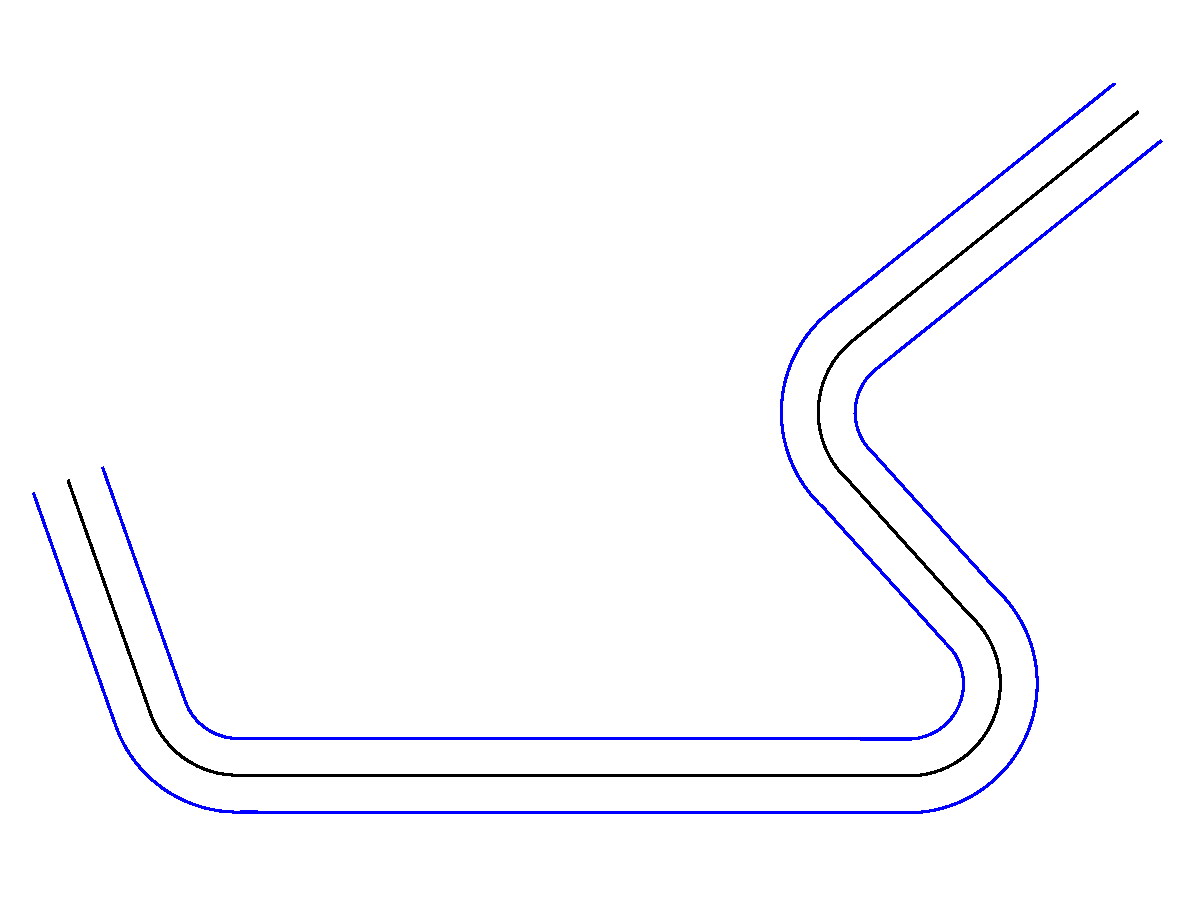
\includegraphics[width=7cm]{5}
  \caption{A `fattened' smoothed polyline; the original smoothed polyline $P_S$ as computed above is drawn in black.  The blue lines represent the same shape offset to either side by an equal distance.}
  \label{fig:fattened-polyline}
\end{figure}
%
The $a'_i$ corresponding to $P_S'$ (with signed offset $d$) can be derived from $P_S$ by adjusting the $r_i$ by $o_id$, where $o_i$ is given by Eq.~\eqref{eq:orientation}.  That is:
%
\begin{equation}
  \label{eq:arc-offset}
  a'_i = \left(c_i, r_i + o_id, \phi^0_i, \phi^1_i\right)
\end{equation}
%
We must also choose new endpoints $p'_0$ and $p'_{n-1}$ for this line;  are the perpendiculars to $n_0$ and $n_{n-2}$ (from Eq.~\eqref{eq:unit-vectors-f}), scaled and added to $p_0$ and $p_{n-1}$, respectively:
%
\begin{align}
  \label{eq:endpoints-prime}
  p'_0 &= p_0 + d \left(\mathbf{n}_0^y, -\mathbf{n}_0^x\right)\\
  p'_{n-1} &= p_{n-1} + d \left(-\mathbf{n}_{n-2}^y, \mathbf{n}_{n-2}^x\right)
\end{align}
%
\subsubsection{Length of offset polylines}
\label{sec:length-offs-polyl}
%
Given a smoothed polyline $P_S$ and an offset $d$, we can express the length of $P'_S$ in terms of Eq.~\eqref{eq:smoothpoly-len}:
%
\begin{align}
  \notag
  L\left(P'_S\right) &= L\left(P\right) + \sum^{n-2}_{i = 1} \left(r_i + o_id\right)\left|\phi^0_i - \phi^1_i\right| - 2\alpha_i\\
  \notag
  &= L\left(P\right) + \sum^{n-2}_{i = 1} r_i\left|\phi^0_i - \phi^1_i\right| - 2\alpha_i + d\sum^{n-2}_{i = 1}  o_i\left|\phi^0_i - \phi^1_i\right|\\
  &= L\left(P_S\right) + d\sum^{n-2}_{i = 1}  o_i\left|\phi^0_i - \phi^1_i\right|
\end{align}
%
\subsubsection{Parametrization and offset smooth polylines}
%
The discussion in Secs.~\ref{sec:length-smooth-polyl} and~\ref{sec:length-offs-polyl} are useful in determining overall lengths, but we may wish to have a method to quickly compute the incremental length along an (offset) smooth polyline; i.e. given $x \in \left[0, 1\right]$, what is $L\left(P_S\right)\left(x\right)$?
%
\subsection{Discrete approximations of smooth polylines}
%
To visually depict a smoothed polyline $P_S$, we may wish to compute a discrete representation.
%
\subsubsection{Polylines}
%
One obvious way to do this is by approximating the shape by a series of lines --- that is to say, a new polyline $P^*$.  See Fig. \ref{fig:disc-polyline}.
%
\begin{figure}
  \centering
  \subfigure[\label{fig:disc-polyline}$P^*$: A polyline approximation of a smoothed polyline $P_S$]{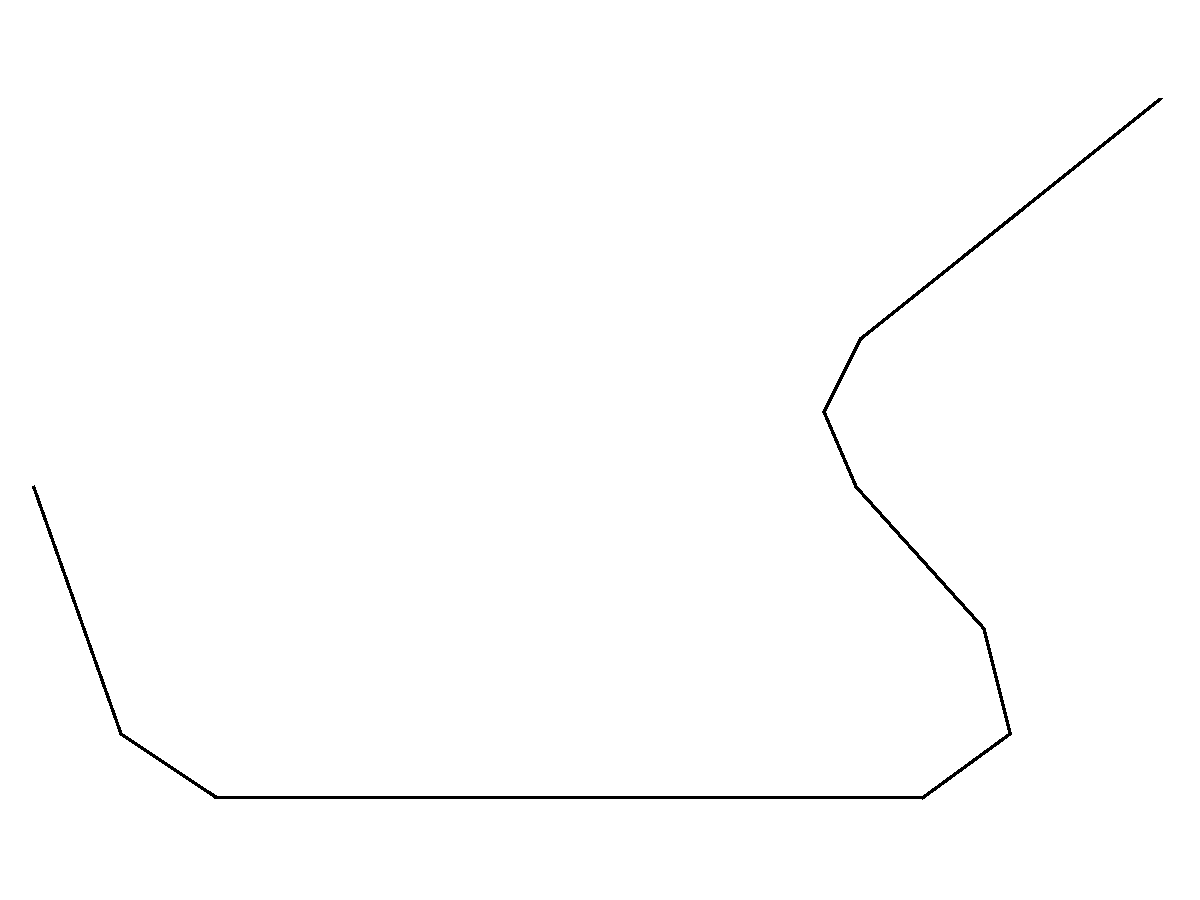
\includegraphics[width=7cm]{6}}\hfill
  \subfigure[\label{fig:mesh-polyline}A triangle mesh approximation of a `fattened' smoothed polyline $P_S$]{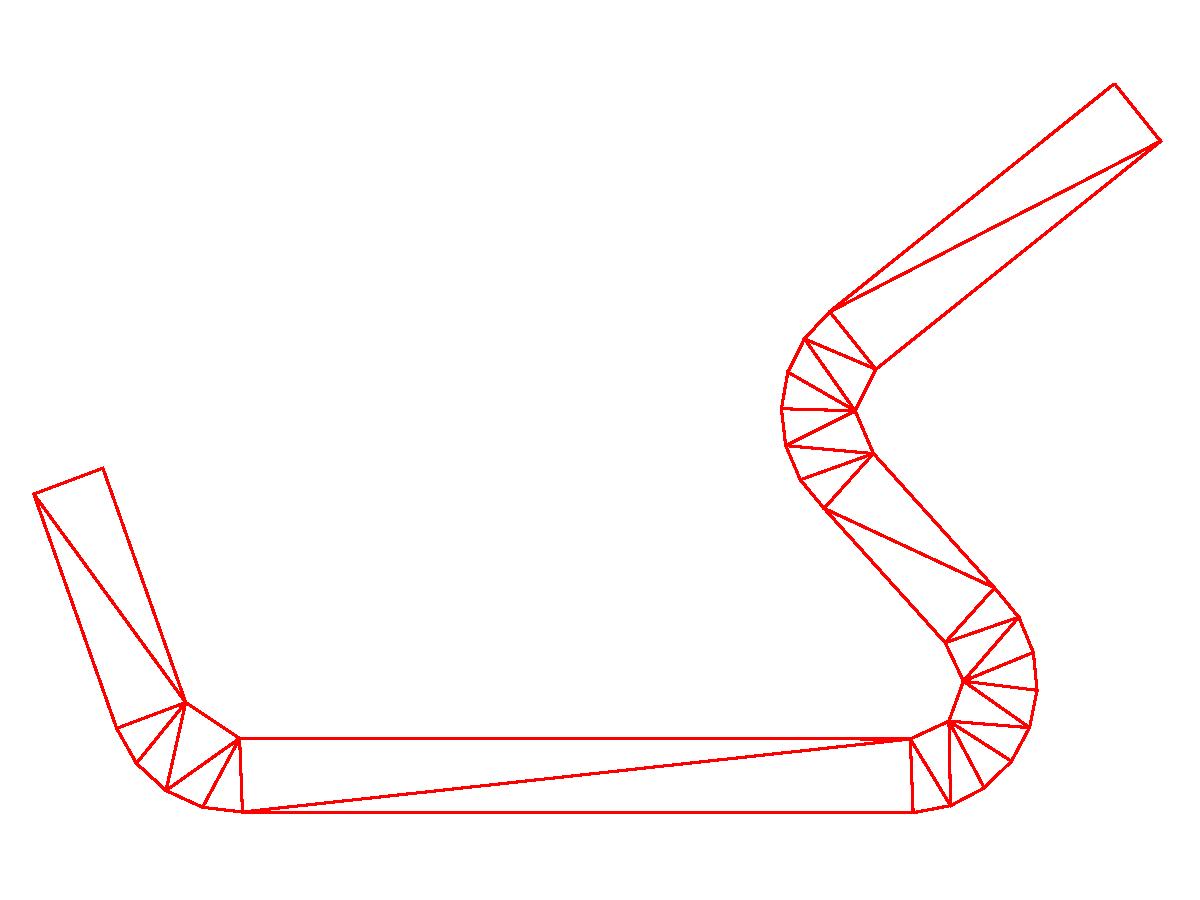
\includegraphics[width=7cm]{7}}
  \caption{Discrete approximations of smoothed polylines}
\end{figure}
%
We must simply approximate each arc $a_i$ with an sequence $\Gamma_i$ of $q_i \in \mathbb{Z}_{>1}$ points, and connect those points with lines.  Then the sequence of $m = 2 + \sum^{n-2}_{i=1} q_i$ points in $P^*$ is simply:
%
\begin{equation}
  \label{eq:p-star}
  P^*_S = \left(p_0, \Gamma^0_0, \ldots, \Gamma^{q_0-1}_0, \ldots, \Gamma^{0}_{n-2}, \ldots, \Gamma^{q_{n-2}-1}_{n-2},  p_{n-2}\right)
\end{equation}
%
We generate each $\Gamma_i$ using the standard parametric form of an arc:
%
\begin{equation}
  \label{eq:arc-segments}
  \Gamma_i = \left(r_i \cos t + c^x, r_i \sin t + c^y\right)
\end{equation}
%
Where $t$ consists of $q_i$ evenly-spaced values in the range $\left[\phi^0_i, \phi^1_i\right]$ (inclusive).
%
\subsubsection{Triangle meshes}
%
A surface representation of a smoothed polygon can be easily computed from a pair of offset polygons (computed as in Sec.~\ref{sec:offset-polylines}).

Given in input smoothed polygon $P_S$ and two smooth polygons offset from $P_S$, order the polygons by offset so that we have a `left' smoothed polygon $P^l_S$ with a lesser offset than the `right' smoothed polygon $P^r_S$.

Now we can use any constrained triangulation technique to compute a planar triangle mesh with $P^l_S$ and $P^r_S$ as the boundaries; see Fig.~\ref{fig:mesh-polyline}.
%
\subsection{Automatic computation of the $r_i$}
%
In Sec.~\ref{sec:formulation-arcs}, we develop the tools to compute the arcs $a_{i}$ for a smoothed polyline $P_{S}$ given a polyline $P$.  Additional information is required for each $a_{i}$, namely either the radius $r_{i}$ or the $\alpha_i$ for that arc.  Given one, we can easily compute the other using Equation~\eqref{eq:radius-alpha}.

Suppose that we have no idea what $r_{i}$ or $\alpha_{i}$ to assign to each arc; we would then like a method for automatically choosing the $r_{i}$ given only $P$ and some simple criteria.  Let's say that we would like to pick the $r_{i}$ such that the quantity
%
\begin{equation}
  \label{eq:optimize-radius}
  \min_{i \in [1, n-2]} r_{i}
\end{equation}
%
is \emph{maximal}.  To begin, we need to know the range of $r_{i}$ (and correspondingly, the $\alpha_{i}$) that may be assigned to each $a_{i}$ given $T_{i}$.
%
\subsubsection{Allowable radii}
\label{sec:allowable-radii}
%
For a given $T_{i}$, the range of suitable radii $r_{i}$ depends on $L_{i-1}$ and $L_i$; we can see in Fig.~\ref{fig:interior-point} that were $r_{i}$ to exceed some quantity, one or both of the points of tangency of the circle on the vectors may lie beyond the length(s) of the vectors --- precisely, we require:
%
\begin{align}
  \label{eq:alphalimit-b}
  \alpha_i &\le L_{i-1}\\
  \label{eq:alphalimit-f}
  \alpha_i &\le L_{i}
\end{align}
%
\paragraph{Lower bound}
%
Obviously, $r_i > 0$ to satisfy the usual meaning of a radius.
%
\paragraph{Upper bound}
%
To derive an upper bound on $r_{i}$ based on the lengths $L_{i-1}$ and $L_i$, we see in Eq.~\eqref{eq:radius-alpha} that $r_{i}$ is linear in $a_{i}$; thus we need only pick the largest $\alpha_i$ that satisfies Eqs.~\eqref{eq:alphalimit-b} and~\eqref{eq:alphalimit-f}.  This is simply
%
\begin{equation}
  \label{eq:alpha-max}
  \alpha^{\max}_i = \min \left\{L_{i-1}, L_{i}\right\}
\end{equation}
%
So for bounds on $r_{i}$, we have
%
\begin{equation}
  \label{eq:rbounds}
  r_{i} \in \left(0, \alpha^{\max}_i \alpha_i\sqrt{\frac{1+\mathbf{n}_i\cdot \mathbf{n}_{i-1}}{1-\mathbf{n}_i\cdot \mathbf{n}_{i-1}}}\right]
\end{equation}
%
\subsubsection{Optimization problem}
\label{sec:optimization}
%
The bounds on $\alpha_i$ given in Equation~\eqref{eq:alpha-max} are valid for a $T_{i}$, but when we are concerned with the $\alpha_i$ for all of the interior points of $P$ we must consider the \emph{available} lengths $L_{i-1}-\alpha_{i-1}$ and $L_{i}+\alpha_{i+1}$.  Since each $r_{i}$ is proportional to the corresponding $\alpha_i$ (Equation~\eqref{eq:radius-alpha}), to satisfy Equation~\eqref{eq:optimize-radius}, we will want each $\alpha_i$ to be as large as possible
%
\begin{align}
  \notag
  \alpha_i &= \min \left\{L_{i-1}-\alpha_{i-1}, L_{i}-\alpha_{i+1}\right\} \\
  \label{eq:alpha-optimize}
  &= \min \left\{L_{i-1}-\alpha_{i-1}, L_{i}-\alpha_{i+1}\right\}
\end{align}
%
Here we define $\alpha_0 = \alpha_{n-1} = 0$.  The optimization problem with constraints from Equation~\eqref{eq:optimize-radius} and objective function given by Equation~\eqref{eq:alpha-optimize} is not amenable to familiar, efficient optimization tools.
%
\subsubsection{Alternate Formulation}
\label{sec:alt-form}
%
Let us relax the constraints in Equation~\eqref{eq:alpha-optimize} to reflect the \emph{legal} states of the $\alpha_i$; we shall leave the maximization of these to the object functions.  Now we have the constraints
%
\begin{equation}
  \label{eq:alpha-length-limit}
  \alpha_i + \alpha_{i+1} \le L_i
\end{equation}
%
where again $\alpha_0 = \alpha_{n-1} = 0$.  We shall find the optimal solution, where we maximize Equation~\eqref{eq:optimize-radius} and then $\sum_i r_i$, through a two-stage process:
%
\begin{enumerate}
\item For each $k\in [1,n-2]$, we solve the linear programming problem to maximize $r_k$ subject to the constraints in Equation~\eqref{eq:alpha-length-limit} and
  %
  \begin{equation}
    \label{eq:ordering-inequality}
    r_k \le r_i \equiv \alpha_k \tan \theta_k \le \alpha_i \tan \theta_i, \quad i \in [1,n-2], i \ne k
  \end{equation}
  %
\item Given the $k$ corresponding to the largest $r_k$ found in step 1, we solve a linear programming problem with the same constraints as in step 1 (namely Equations~\eqref{eq:alpha-length-limit} and~\eqref{eq:ordering-inequality}) but now maximizing $\sum_i r_i = \sum_i \alpha_i \tan \theta_i$.
\end{enumerate}
%
\end{document}
%
%%% Local Variables:
%%% mode: latex
%%% TeX-master: t
%%% End:
